\documentclass[preprint, 10pt]{sigplanconf}

\usepackage{amsmath}
\usepackage{booktabs}
\usepackage{longtable}
\usepackage{tikz}
\usepackage{listings}
\usetikzlibrary{positioning}
\newcommand{\cL}{{\cal L}}
\newcommand{\colAwidth}{0.1\textwidth}
\newcommand{\colBwidth}{0.34\textwidth}
\begin{document}

\special{papersize=8.5in,11in}
\setlength{\pdfpageheight}{\paperheight}
\setlength{\pdfpagewidth}{\paperwidth}

\conferenceinfo{Onward! '16}{October 30--November 4, 2016, Amsterdam, Netherlands}
\copyrightyear{2016}
\copyrightdata{978-1-nnnn-nnnn-n/yy/mm}
\copyrightdoi{nnnnnnn.nnnnnnn}

% Uncomment the publication rights you want to use.
%\publicationrights{transferred}
%\publicationrights{licensed}     % this is the default
%\publicationrights{author-pays}

\titlebanner{banner above paper title}        % These are ignored unless
\preprintfooter{short description of paper}   % 'preprint' option specified.

\title{Title Text}
\subtitle{Subtitle Text, if any}

\authorinfo{Dan Szymczak}
           {McMaster University}
           {szymczdm@mcmaster.ca}
\authorinfo{Jacques Carette\and Spencer Smith}
           {McMaster University}
           {carette@mcmaster.ca / smiths@mcmaster.ca}

\maketitle

\begin{abstract}
This will be filled in once we're done drafting. For now I'm putting in a solid
block of text that will let me ramble on for a while when it comes down to the
final abstract. Programmers are like gods of tiny universes. They create worlds
according to their rules. If we think of software artifacts (that is, all
documentation, build instructions, source code, etc.) as their own tiny worlds,
a universe takes shape. Now think about what would happen if the laws of that
universe were inconsistent between worlds. What if the laws of thermodynamics
fundamentally changed as soon as you left Earth? Say goodbye to space travel.
Keeping artifacts consistent with each other is hugely important in the software
world, and Drasil aims to ensure it...
\end{abstract}

\category{CR-number}{subcategory}{third-level}

% general terms are not compulsory anymore,
% you may leave them out
%\terms
%term1, term2

\keywords
Literate software, knowledge capture, traceability, software engineering,scientific 
computing, artifact generation, software quality

\section{Introduction}
\label{sec:Intro}

We want to make better software.  In particular, we are interested in
increased maintainability, traceability, reproducibility, verifiability, and
reusability.  Our approach is to invest (much) more in the short-term to provide
outstanding long-term benefits. This is the fundamental trade-off in
our work: we expect our methods to work very well for domains which are 
well understood with known (but potentially enormous) design spaces.  We do
not claim to tackle areas of software development where methodologies such
as agile are well-suited.  But we firmly believe that there are domains --
such as safety-critical applications -- where agile is not only ill-suited,
it would be downright unprofessional to use such a methology in that setting.

Rather than talk in vague generalities, we will pick Scientific Computation
(SC) for illustrative purporses throughout this paper.  But the fundamental
ideas (and, in fact, our framework) should be applicable to any software
domain which has well-established theoretical underpinnings, and a well
understood translation of the theory into effective code.  SC is particularly
well-suited as it is also replete with \emph{program families}.

We believe that Knuth's Literate Programming (LP)~\cite{Knuth1984} contains
some fundamental insights, but is too restricted (i.e. just to code).  Rather
than restrict LP to just source code, we want to apply it to all software
artifacts (requirements and design documents, source files, test cases, build
instructions, user manuals, etc.) from a singular common knowledge base.

We want to break away from the LP idea of ``one source'', instead introducing
the idea of ``common knowledge'' libraries for problems that come up regularly.
For example: the theory behind heat transfer including the conservation of
energy equations would be in a ``common knowledge'' library. We could also see
the idea of the Syst\`{e}me International (SI) Units as another piece of
``common knowledge''.

We also very much want to keep the idea of ``chunks'' and assemble everything
from chunks. How we do that will be discussed in more detail in
Section~\ref{sec:Drasil}.

We intend to make working on program families trivial for the cost of losing the
capability to create ``local hacks'' to ``just get things working''.

Another disclaimer before we go further: none of the ideas presented
in this paper are new. We are building on a very longstanding history of work,
and not being particularly creative with the ideas therein. Knuth himself even
said that ``I have simply combined a bunch of ideas that have been in the air
for a long time'' when he coined LP~\cite{Knuth1984}. We are, however, taking old
ideas and breaking them down into something practical that we can work with. We
want to \emph{do} something, not spend years stuck in the design phase.

Others have done similar work (which we will get into in Section~\ref{sec:bg}),
but they did not achieve the results we are envisioning. They either set their
aims on other targets, spent too long creating a grand design and ended up
without any real, practical results, or they simply were not brave enough to
break things down into the smallest necessary chunks.

We believe that we have assembled the right ideas to achieve our vision.
The overall success or failure of our approach hinges on the idea of a stable,
well understood knowledge base. Without that we might as well give up and go
home. If we do not understand the fundamentals behind the software we intend to
create, then we will be unable to properly encapsulate that fundamental
knowledge for use in our framework (effectively getting us nowhere).

As it stands, we are on a (not so) humble, practical route to achieving our
goals and improving the overall quality of software.

\section{Drasil}
\label{sec:Drasil}

Our framework is called Drasil (shortened from \emph{Yggdrasil} from Norse
Mythology, which is also known as the \emph{world tree}). It is currently being
developed through a practical, example-driven approach in an effort to bring our
vision to life. There are three main ideas driving Drasil's development:

\begin{enumerate}
\item Organize the knowledge base -- We want a knowledge base that we can
structure conceptually (i.e. keep knowledge for a certain class of problems
together). This is where chunks come into play: each chunk encapsulates a single
piece of knowledge like a concept or a quantity. We want to break our knowledge
base down into the smallest possible pieces.

\item Use recipes to create artifacts -- We can think of each artifact in our
software project as a different view of our knowledge base. We want to use
recipes to specify exactly what information from the knowledge base is necessary
for each artifact, and how that information should be displayed. For many
artifacts we would like to have a standard recipe which can be quickly
customized for the current problem and that is how we will avoid duplicating
knowledge.

\item Remove technology constraints -- We want to be able to create our software
without worrying about the underlying technical constraints of our display or
specification technology, programming language(s), etc. Anyone using Drasil
should be able to work with the knowledge base and their recipes, then simply
set their output technology and have the generator take care of all the
technical details.
\end{enumerate}

We argue that by implementing Drasil around these ideas, we can see drastic
improvements in software quality. In fact, using a generative approach we can
avoid certain problems altogether. One obvious and recurring problem that comes
to mind when upgrading software is ``feature creep'' or ``software
bloat''~\cite{AmselEtAl2011}. With Drasil, a software upgrade will actually be a
completely new piece of software that includes the previously desired
functionality as well as the new upgrades. We will discuss further improvements
in more detail after our example in Section~\ref{subsec:example}.

\subsection{Drasil's current implementation}
\label{subsec:current}

Fundamentally, Drasil must be able to capture knowledge and produce different
views of that knowledge. With our current implementation we have each individual
piece of knowledge as a named \emph{chunk}. We are then able to manipulate our
chunks through the use of a \emph{recipe}. Our \emph{generator} interprets the
recipes to produce the final desired view. This view represents one of the many
software artifacts mentioned in Section~\ref{sec:Intro}.

As mentioned, we capture knowledge into named chunks, of which there
are several varieties. Actually, we have a hierarchy of chunk types, where each
new chunk encapsulates more than the previous one(s) (see
Figure~\ref{fig:chunks} for an idea). The most basic \emph{chunk} represents a
named piece of information. Above that we have named \emph{concepts} which
introduce some descriptive information.

A \emph{quantity} is a concept that has a symbolic representation, we can refer
to the quantity by either its name or symbol. In a similar vein are
\emph{units}, %need something more here -- (which encapsulates the units
%attached to a concept)?? 
and \emph{relation chunks} (which add the idea of a
relation between some other pieces of knowledge).

In an SC context, most of the knowledge we work with is represented as a
quantity with some units, in other words a \emph{unital} chunk. Expanding on
that, we can actually calculate values for many of these unital concepts. As
such, we have \emph{eqchunks} which allow us to capture the equation along with
everything else included in a unital chunk.

\begin{figure}
\begin{center}
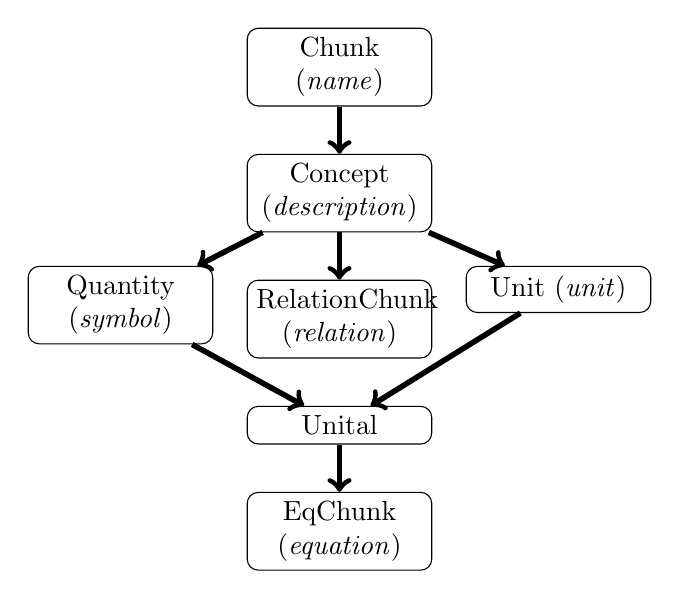
\begin{tikzpicture}[node distance=6mm]
  \tikzstyle{every node}=[draw,shape=rectangle, rounded corners,
    text width=6em, text centered];
  \node (ch)                     {Chunk (\emph{name})};
  \node (co) [below = of ch]       {Concept (\emph{description})};
  \node (qu) [below left = of co]  {Quantity (\emph{symbol})};
  \node (rc) [below = of co]		   {RelationChunk (\emph{relation})};
  \node (u ) [below right = of co] {Unit (\emph{unit})};
  \node (uc) [below = of rc] 		{Unital};
  \node (eq) [below = of uc]		   {EqChunk (\emph{equation})};

  \draw [->, line width=2pt] (ch) -- (co);
  \draw [->, line width=2pt] (co) -- (qu);
  \draw [->, line width=2pt] (co) -- (rc);
  \draw [->, line width=2pt] (co) -- (u );
  \draw [->, line width=2pt] (qu) -- (uc);
  \draw [->, line width=2pt] (u ) -- (uc);
  \draw [->, line width=2pt] (uc) -- (eq);
\end{tikzpicture}
\end{center}
\caption{Our current chunk design}
\label{fig:chunks}
\end{figure}

Now with the means to encapsulate knowledge, we can turn our attention to our
recipes. The recipes are implemented using a combination of embedded Domain
Specific Languages (DSLs) in Haskell. We have currently implemented the
following DSLs:

\begin{enumerate}
\item Expression language -- A simple expression language that allows us to
capture knowledge relating to equations and mathematical operations. It
includes, but is not limited to, operations such as addition, multiplication,
negation, derivation, and exponentiation.

\item Expression layout language -- A micro-scoped language for describing how
expressions should appear. Expressions may need to use subscripts, superscripts,
concatenated symbols, etc. to be properly displayed.

\item Document layout language -- A macro-scoped language for describing how
large-scale layout objects (tables, sections, figures, etc.) should appear.

\item C Representation Language -- A DSL for representing parts of the C
programming language inside the Drasil framework. This allows the generator to
produce working C code.

\item \LaTeX Representation Language -- A DSL for representing \LaTeX code
inside of Drasil.

\item HTML Representation Language -- A DSL for representing HTML within Drasil.
\end{enumerate}

Of the DSLs mentioned, we only actually have to write our recipes using three of
them. Each of the representation languages are used strictly by the generator as
an intermediary in the production of our desired views. We write our recipes
using the document layout language, expression layout language, and expression
language. We will discuss the particulars of each of these in more depth during
our example (Section~\ref{subsec:example}).

The last piece of the puzzle is the generator. We use it to interpret the
recipes, create intermediary representations of our desired views, and then
pretty-print them.

\subsection{Drasil in Action} \label{subsec:example}
For this section we will take a look at a simplified version of a Software
Requirements Specification (SRS) for a fuel pin in a nuclear reactor (for more
information on that particular SRS see~\cite{SmithAndKoothoor2016}).

Starting off we will look at one specific term: $h_c$. In this example, $h_c$
represents the convective heat transfer coefficient between the clad and
coolant. The data definition for $h_c$ from the original SRS can be seen in
Figure~\ref{fig:h_c}.

\begin{figure}
~\newline \noindent \begin{minipage}{\textwidth}
\begin{tabular}{p{\colAwidth} p{\colBwidth}}
\toprule \textbf{Number} & \textbf{DD2 \label{hc}}
\\ \midrule 
Label & 
$h_{c}$
\\ \midrule
Units & $ML^0t^{-3}T^{-1}$\\ \midrule
SI Units & $\mathrm{\frac{kW}{m^{2o}C}}$\\ \midrule
Equation & $h_{c}$ =$
\frac{2k_{c}h_{b}}{2k_{c}+\tau_{c}h_{b}}$\\ \midrule
Description & $h_{c}$ is the convective heat transfer coefficient between clad
and coolant
\newline
$k_{c}$ is the
clad conductivity \newline
$h_{b}$ is the
initial coolant film conductance \newline
$\tau_{c}$ is the
clad thickness 
\newline
%NOTE: Equation taken from the code\\ \midrule  Sources & source code \\ \bottomrule 
\end{tabular} \end{minipage}\\ 
\caption{Data definition for $h_c$ from the fuel pin SRS}
\label{fig:h_c}
\end{figure}

The data definition of $h_c$ displays some interesting knowledge. It gives us
the name for a concept, its description, a symbol to use for easier reference,
its (SI) units, and its defining equation. Encapsulating all of this knowledge
into a chunk is not very difficult as shown in Figure~\ref{fig:h_cChunk}. Note
that the equation for $h_c$ is written in our expression language (Expr) and it
also includes references to chunks that $h_c$ depends on. These will come into
play when we create the description for $h_c$ in the generated view, but we do
not need to worry about them right now as that knowledge is stored elsewhere.
The units for $h_c$ are defined by a piece of common knowledge known as
\verb|heat_transfer|.

\begin{figure}
\begin{lstlisting}[frame=single, showstringspaces=false, basicstyle=\small]
h_c_eq :: Expr
h_c_eq = 2*(C k_c)*(C h_b) /
  (2*(C k_c) + (C tau_c)*(C h_b))

h_c :: EqChunk
h_c = fromEqn "h_c" 
 "convective heat transfer coefficient
    between clad and coolant"
 (sub h c) heat_transfer h_c_eq
\end{lstlisting}
\caption{The $h_c$ chunk in Drasil}
\label{fig:h_cChunk}
\end{figure}

On the topic of common knowledge, we can show an example alluded to previously,
that of the SI unit library. The seven base SI units captured in Drasil are
shown in Figure~\ref{fig:si_units}. The SI unit library also contains several
derived units (for example: centigrade which is derived from kelvin) which we
make use of later on in our example. The knowledge behind each unit and (in the
case of derived units) their relation to the base units is captured in the
relevant chunks.

\begin{figure*}
\begin{lstlisting}[frame=single, showstringspaces=false]
metre, second, kelvin, mole, kilogram, ampere, candela :: FundUnit
metre    = fund "Metre"    "length (metre)"               "m"
second   = fund "Second"   "time (second)"                "s"
kelvin   = fund "Kelvin"   "temperature (kelvin)"         "K"
mole     = fund "Mole"     "amount of substance (mole)"   "mol"
kilogram = fund "Kilogram" "mass (kilogram)"              "kg"
ampere   = fund "Ampere"   "electric current (ampere)"    "A"
candela  = fund "Candela"  "luminous intensity (candela)" "cd"
\end{lstlisting}
\caption{The seven funamental SI Units in Drasil}
\label{fig:si_units}
\end{figure*}

Now that we've shown a bit of knowledge capture, you may be wondering how to use
it. This is where the recipes come in. Figure~\ref{fig:recipe} shows a portion
of the recipe for creating our intended SRS view. The body of the simplified SRS
is composed of three sections: \verb|s1|, \verb|s2|, and \verb|s3|. We then show
the definition of the first section (omitting the others for brevity) which is
titled "Table of Units" and includes an introductory paragraph and a table. This
table simply extracts the symbol and description information from the SI units
to display them in our view. It should be fairly obvious at this point, but
these macro-scale layout objects (sections, tables, paragraphs, etc.) are
specified using our document layout language.

\begin{figure}[tb]
\begin{lstlisting}[frame=single, 
  showstringspaces=false, basicstyle=\scriptsize]
srsBody = srs [h_g, h_c] "Spencer Smith" [s1,s2,s3]

s1 = Section (S "Table of Units") [intro, table]

table = Table 
 [S "Symbol", S "Description"] (mkTable
   [(\x -> Sy (x ^. unit)),
    (\x -> S (x ^. descr)) ] si_units)

intro = Paragraph (S "Throughout this ...")
\end{lstlisting}
\caption{A portion of our simplified SRS recipe}
\label{fig:recipe}
\end{figure}

With our recipe in place, we are now able to run it through the generator and
see what it spits out. We've included the three sections of this simplified SRS
in Appendix~\ref{appendix:SRS}, and what you see there is the typeset version of
the generated LaTeX code. We are also able to output our view as an HTML
document (Figure~\ref{fig:HTML_s1}).

\begin{figure}
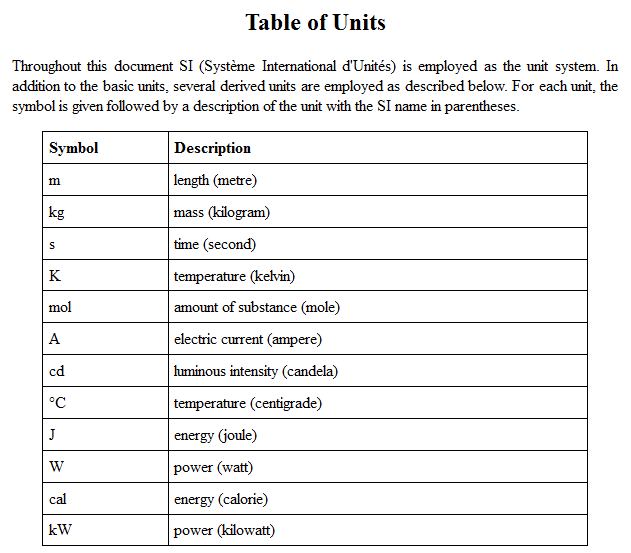
\includegraphics[scale=0.5]{HTML_s1.png}
\caption{Section 1 of the generated SRS (HTML version)}
\label{fig:HTML_s1}
\end{figure}

Now if you recall the data definition from Figure~\ref{fig:h_c}, we will show
the painstaking amount of work it takes to create (almost) that exact same
table:

\begin{lstlisting}
s3_dd2 = Definition (Data h_c)
\end{lstlisting}

Again looking to the appendix, or to the HTML output (Figure~\ref{fig:HTML_s3} for
the data definition), it should be easy to see that the recipe handled all of
the layout details. The recipe actually goes one step further in that it found
all of the chunk's dependencies and built the description by finding the
appropriate knowledge related to the other chunks. This is configurable in that
we can include short descriptions or verbose descriptions at this point in time.

\begin{figure}
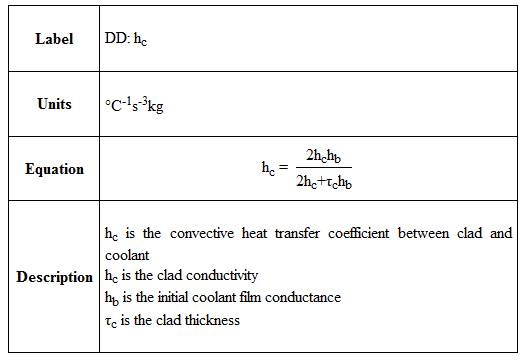
\includegraphics[scale=0.6]{HTML_s3.png}
\caption{Generated SRS data definition (HTML version)}
\label{fig:HTML_s3}
\end{figure}

One last thing we'd like to show is the source code generation. The recipe is
fairly straightforward in that we have:

\begin{lstlisting}
codesample = CodeBlock (toCode CLang Calc h_c)
\end{lstlisting}

All that says is \verb|codesample| is a block of code in the C language that
calculates the value of $h_c$. Currently the only implemented output language is
C, but we are planning to implement more and are designing around that coming
change. The generator output for \verb|codesample| ends up looking like:

\begin{lstlisting}[frame=single, 
  showstringspaces=false, basicstyle=\scriptsize]
double calc_h_c(double k_c, double h_b, double tau_c){
    return (2 * k_c * h_b / (2 * k_c + tau_c * h_b));
}
\end{lstlisting}

This is a fairly trivial piece of code, but it is a good example of how the
source can be generated from the knowledge encapsulated in a chunk.

\subsection{Advantages and Disadvantages}

Zero knowledge duplication -- look at all of the previous figures (or
Appendix~\ref{appendix:SRS}) and how many times knowledge has been copied into
different places within one software artifact. Now imagine how many times that
knowledge appears across all software artifacts. Generation avoids the problem
of needing to manually duplicate all of that information. It also ensures that
should a piece of knowledge need to be updated, the updates will propagate
throughout all of the artifacts automatically.

\clearpage
\onecolumn
\appendix
\section{Simplified SRS}
\label{appendix:SRS}
Here we see the typeset output of the LaTeX code for the simplified SRS example:

\section*{Table of Units}
\label{Sec:ToU}
Throughout this document SI (Syst\`{e}me International
d'Unit\'{e}s) is employed as the unit system. In addition to
the basic units, several derived units are employed as
described below. For each unit, the symbol is given followed
by a description of the unit with the SI name in
parentheses.
\begin{longtable}{l p{8.5cm}}
Symbol & Description\
\\
m & length (metre)\
\\
kg & mass (kilogram)\
\\
s & time (second)\
\\
K & temperature (kelvin)\
\\
mol & amount of substance (mole)\
\\
A & electric current (ampere)\
\\
cd & luminous intensity (candela)\
\\
${}^{\circ}$C & temperature (centigrade)\
\\
J & energy (joule)\
\\
W & power (watt)\
\\
cal & energy (calorie)\
\\
kW & power (kilowatt)\
\\
\label{Table:ToU}
\end{longtable}
\section*{Table of Symbols}
\label{Sec:ToS}
The table that follows summarizes the symbols used in this document along with
their units. The choice of symbols was made with the goal of being consistent
with the nuclear physics literature and that used in the FP manual. The SI units
are listed in brackets following the definition of the symbol.
\begin{longtable}{l l p{8.5cm}}
Symbol & Description & Units\
\\
$h_{g}$ & effective heat transfer coefficient between clad
and fuel surface & ${}^{\circ}$C$^{-1}$s$^{-3}$kg\
\\
$h_{c}$ & convective heat transfer coefficient between clad
and coolant & ${}^{\circ}$C$^{-1}$s$^{-3}$kg\
\\
\label{Table:ToS}
\end{longtable}
\section*{Data Definitions}
\label{Sec:DD}
~\newline \noindent \begin{minipage}{.7\textwidth}
\begin{tabular}{p{0.2\textwidth} p{0.73\textwidth}}
\toprule \textbf{Refname} & \textbf{DD:h.g}
\label{DD:h.g}
\\ \midrule \\
Label & $h_{g}$
\\ \midrule \\
Units & ${}^{\circ}$C$^{-1}$s$^{-3}$kg
\\ \midrule \\
Equation & $h_{g}$ = $\frac{2h_{c}h_{p}}{2h_{c}+\tau{}_{c}h_{p}}$
\\ \midrule \\
Description & $h_{g}$ is the effective heat transfer
coefficient between clad and fuel surface
\\ \bottomrule \end{tabular}
\end{minipage}\\
~\newline \noindent \begin{minipage}{.7\textwidth}
\begin{tabular}{p{0.2\textwidth} p{0.73\textwidth}}
\toprule \textbf{Refname} & \textbf{DD:h.c}
\label{DD:h.c}
\\ \midrule \\
Label & $h_{c}$
\\ \midrule \\
Units & ${}^{\circ}$C$^{-1}$s$^{-3}$kg
\\ \midrule \\
Equation & $h_{c}$ = $\frac{2h_{c}h_{b}}{2h_{c}+\tau{}_{c}h_{b}}$
\\ \midrule \\
Description & $h_{c}$ is the convective heat transfer
coefficient between clad and coolant
\\ \bottomrule \end{tabular}
\end{minipage}\\

%\acks
%
%Acknowledgments, if needed.

% We recommend abbrvnat bibliography style.
\clearpage
\twocolumn
\bibliographystyle{abbrvnat}
\bibliography{drasil}
%
% The bibliography should be embedded for final submission.
%
%\begin{thebibliography}{}
%\softraggedright
%
%\bibitem[Smith et~al.(2009)Smith, Jones]{smith02}
%P. Q. Smith, and X. Y. Jones. ...reference text...
%
%\end{thebibliography}


\end{document}
